%----------------------------------------
% Preamble to set up the document
%----------------------------------------
\documentclass{article}

% set up packages (you shouldn't need to touch this)
\usepackage{graphicx}  % required to insert images
\usepackage{hyperref}  % for hyperlinks
\usepackage[svgnames]{xcolor}  % to change hyperlink colors
\usepackage{amsmath}
\usepackage{amssymb}
\colorlet{linkcolour}{DarkBlue}
\hypersetup{colorlinks=true, linkcolor=linkcolour, citecolor=linkcolour, urlcolor=linkcolour,}

% Margins
\topmargin=-0.45in
\evensidemargin=0in
\oddsidemargin=0in
\textwidth=6.5in
\textheight=9.0in
\headsep=0.25in

% use a sans serif font
\renewcommand{\familydefault}{\sfdefault}

%----------------------------------------
% Step 1: Edit the lecture title
%----------------------------------------
\title{
Lecture 7:  Regression \\  % Lecture title
Modeling Social Data, Spring 2019 \\   % Course title
Columbia University                    % School
}

%----------------------------------------
% Step 2: Edit your name and the date
%----------------------------------------
\author{Bhavya Shahi (bs3118)}                     % Scribe's name
\date{March 8, 2019}                % Lecture date

\begin{document}

\maketitle


%----------------------------------------
% Step 3:
% Rename uni.tex to match your uni,
% edit the filename accordingly below,
% and put your notes in this file
%----------------------------------------
%----------------------------------------
% Write your notes here
%----------------------------------------
\section{Reproducibility}
As discussed in the previous class, there is currently a crisis of reproducibility and replication. To counter this, there a few guidelines we should follow before we publish research. 
\begin{itemize}
    \item Read all the pertinent literature, as you may not be the first person to have this idea. Literature surveys also help in understanding our problem better
    \item Formulate your study
    \item Run a pilot to test the study
    \item Analyze the results of the study
    \item Revise your study based on this analysis 
    \item Calculate the power of your study, to define the effect and population size needed 
    \item Pre-regiser plans for your study online. This helps in reviewing your process, and ensures that you cannot lie about the results later on.
    \item Run your study 
    \item Create a detailed and reproducible report using the makefile templates define during the pilot study
    \item Think critically about your results
    \item Disclose everything you did during the study, including data collection, preprocessing etc. 
    
\end{itemize}
Other good practices for reproducibility include:
\begin{itemize}
    \item Use \href{https://www.mturk.com/}{Mechanical Turk} to collect data since it is reliable and quick
    \item Running a pilot study first
    \item Creating a framework to analyse the data that can be easily reproduced based on the pilot study 
    \item To ensure that the subjects in the study understand the questions, we should add some questions as sanity checks. 
    \item We could also use timestamps of the data collected to remove any bots.
\end{itemize}
Also, we should remember: \newline

Standard deviation: The variation in the data (this remains constant no matter how many samples we choose)\newline

Standard error: This represents how far the sample mean is from the population mean. Thus, if we take more number of samples, we can reduce this. 

\section{Regression}
Regression is used to estimate the relationship between variables. It can be used to summarize the data, predict future data, and explain relationships within the data. We need to find a balance between understanding out current data, and being able to generalize in a way that we can also predict future outcomes. The task is to find a function to do this.
The notes below show the how the task is defined.
\subsection{Task}
\begin{figure}[!ht]
  \begin{center}
    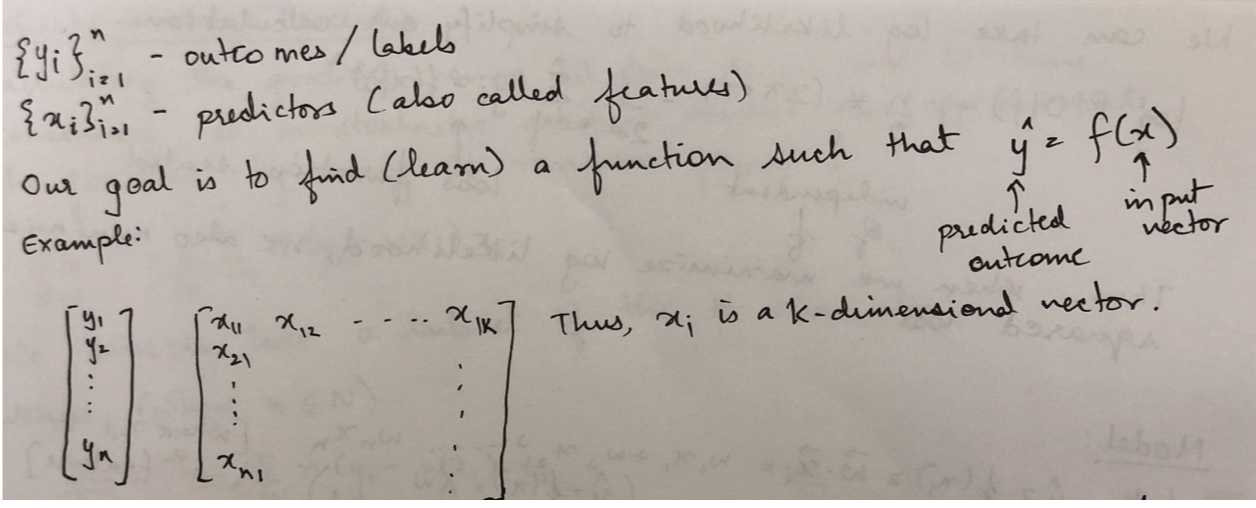
\includegraphics[scale=0.8]{figures/1.png}
    \caption{Defining the task }
    \label{fig:1}
  \end{center}
\end{figure}
\subsection{Loss functions}
We then define loss functions to evaluate our function.
The notes below show the how the task is defined.
\begin{figure}[!ht]
  \begin{center}
    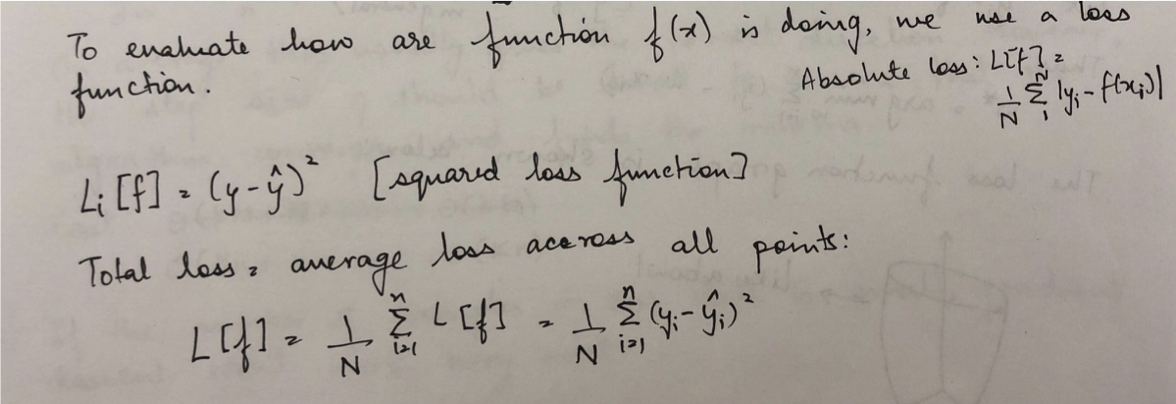
\includegraphics[scale=0.8]{figures/2.png}
    \caption{Define loss functions }
    \label{fig:2}
  \end{center}
\end{figure}
\newpage
\subsection{MLE}
Maximum Likelihood Estimator is used to find how to minimize loss.
\begin{figure}[!ht]
  \begin{center}
    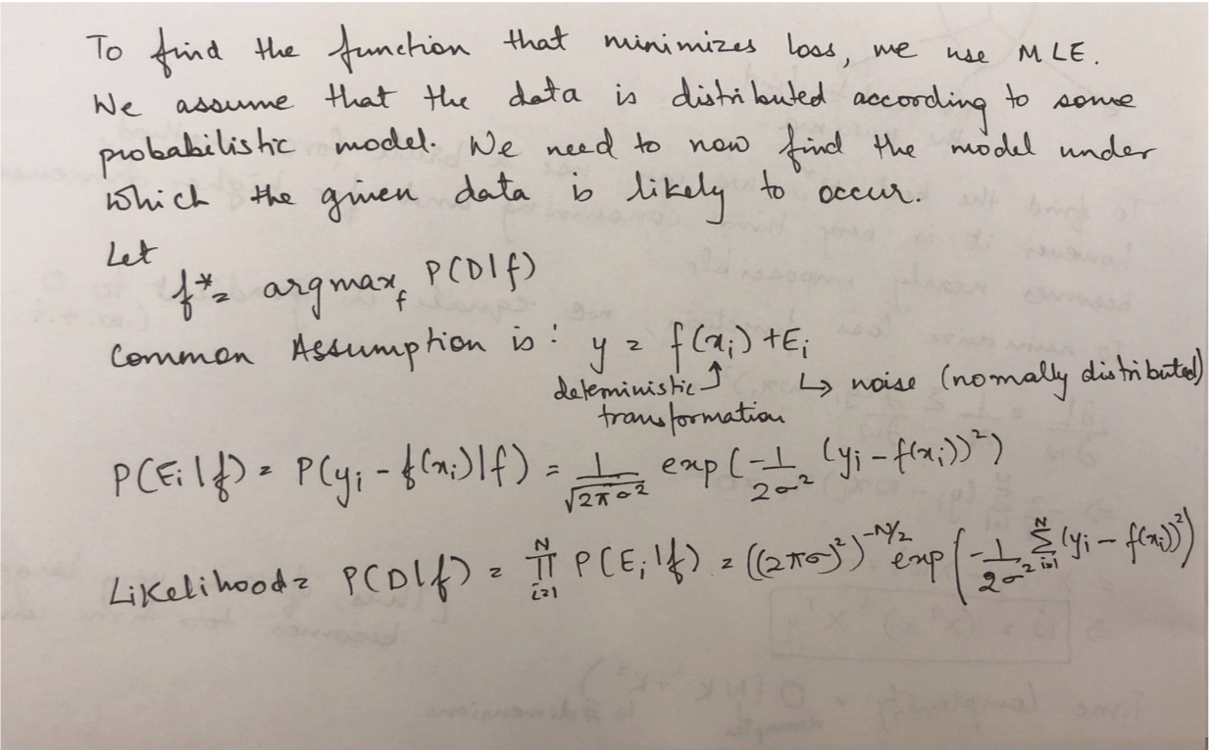
\includegraphics[scale=0.8]{figures/3.png}
    \caption{MLE }
    \label{fig:3}
  \end{center}
\end{figure}

\begin{figure}[!ht]
  \begin{center}
    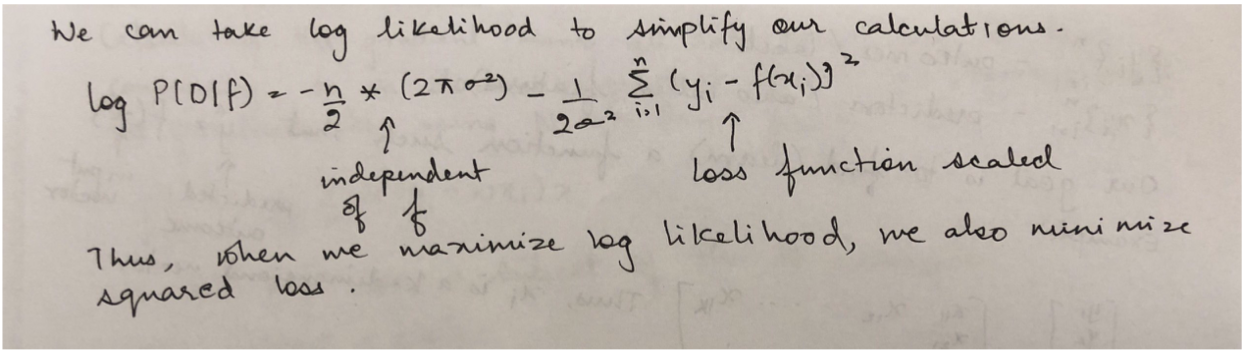
\includegraphics[scale=0.8]{figures/4.png}
    \caption{MLE }
    \label{fig:4}
  \end{center}
\end{figure}
\newpage
\subsection{Finding f(x)}
We then define the regression model in terms of weights. To find the best possible value of the weight vector, we can use three main methods: Normal equations (shown in Figure \ref{fig:5}), Gradient Descent (Figure \ref{fig:6}), and Stochastic Gradient Descent (shown in Figure \ref{fig:7})
\begin{figure}[!ht]
  \begin{center}
    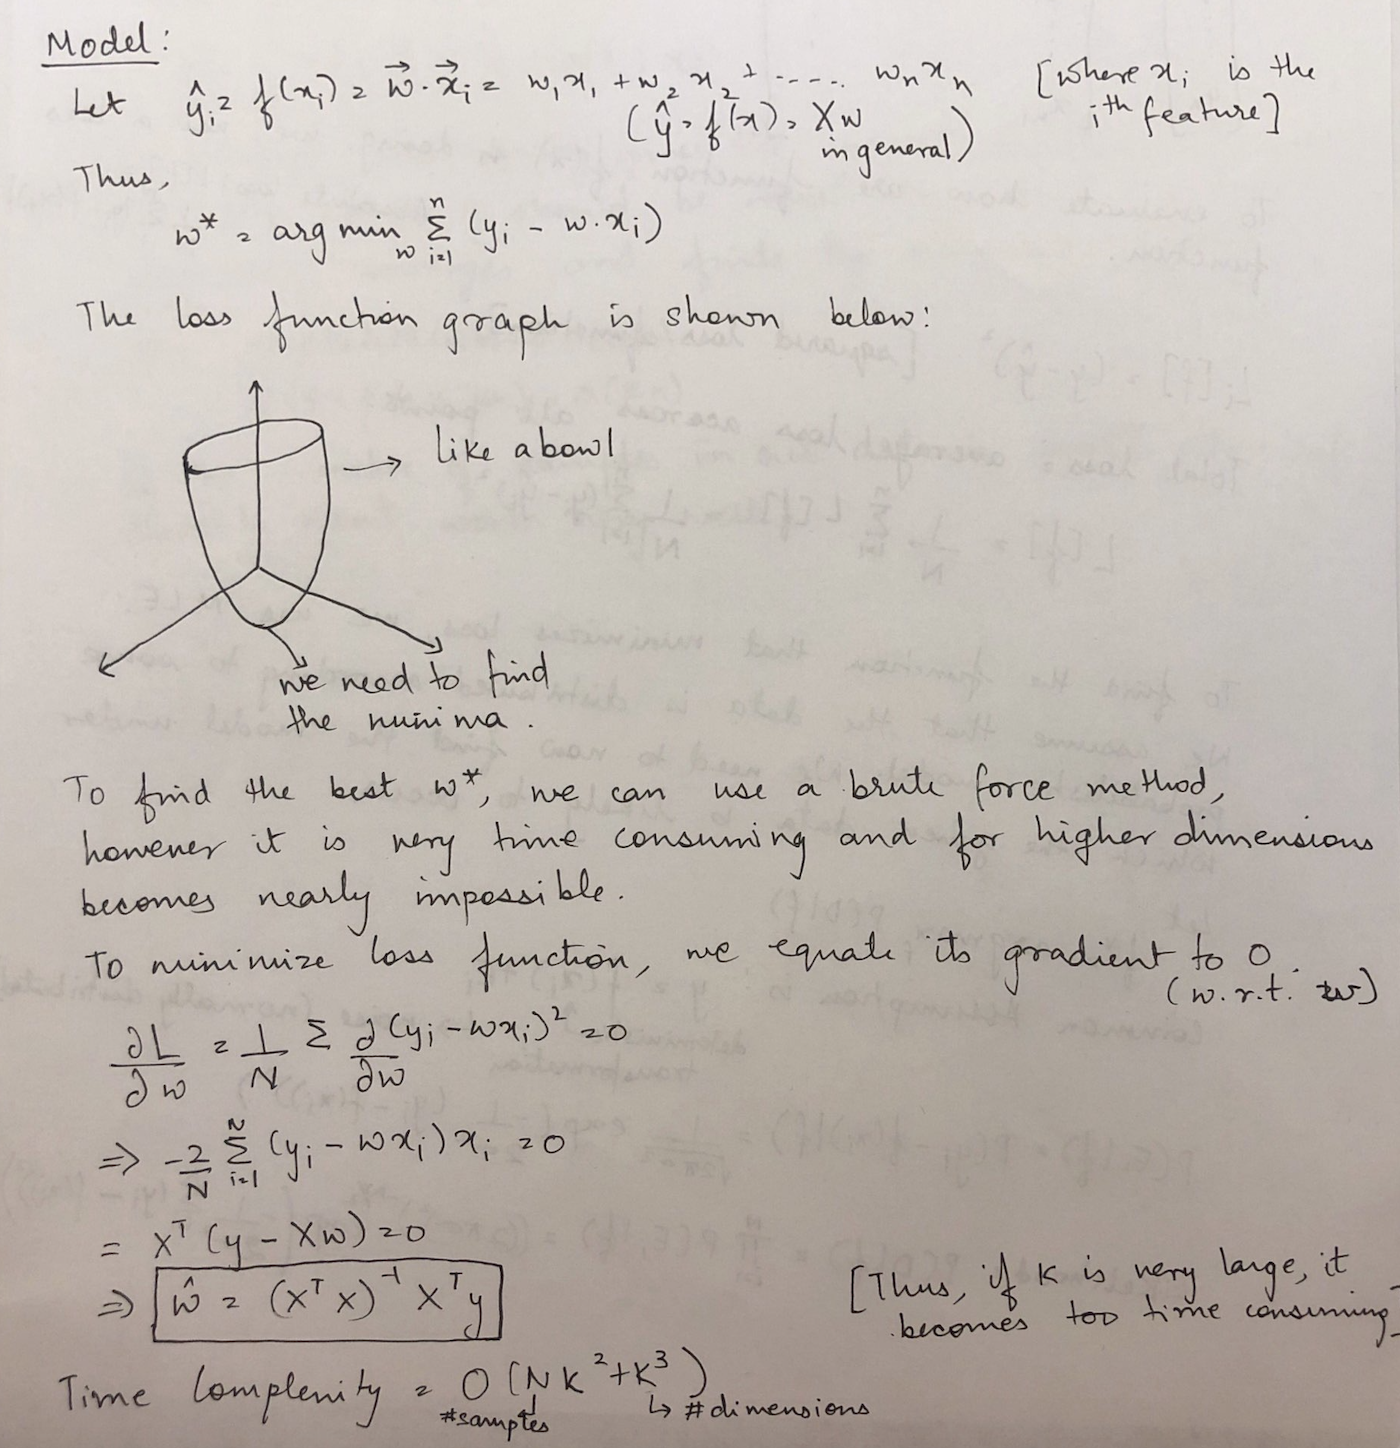
\includegraphics[scale=0.7]{figures/5.png}
    \caption{Defining and determining f(x) }
    \label{fig:5}
  \end{center}
\end{figure}

\newpage
\subsection{Gradient Descent}
Gradient descent can be used to estimate the w vector.

\begin{figure}[!ht]
  \begin{center}
    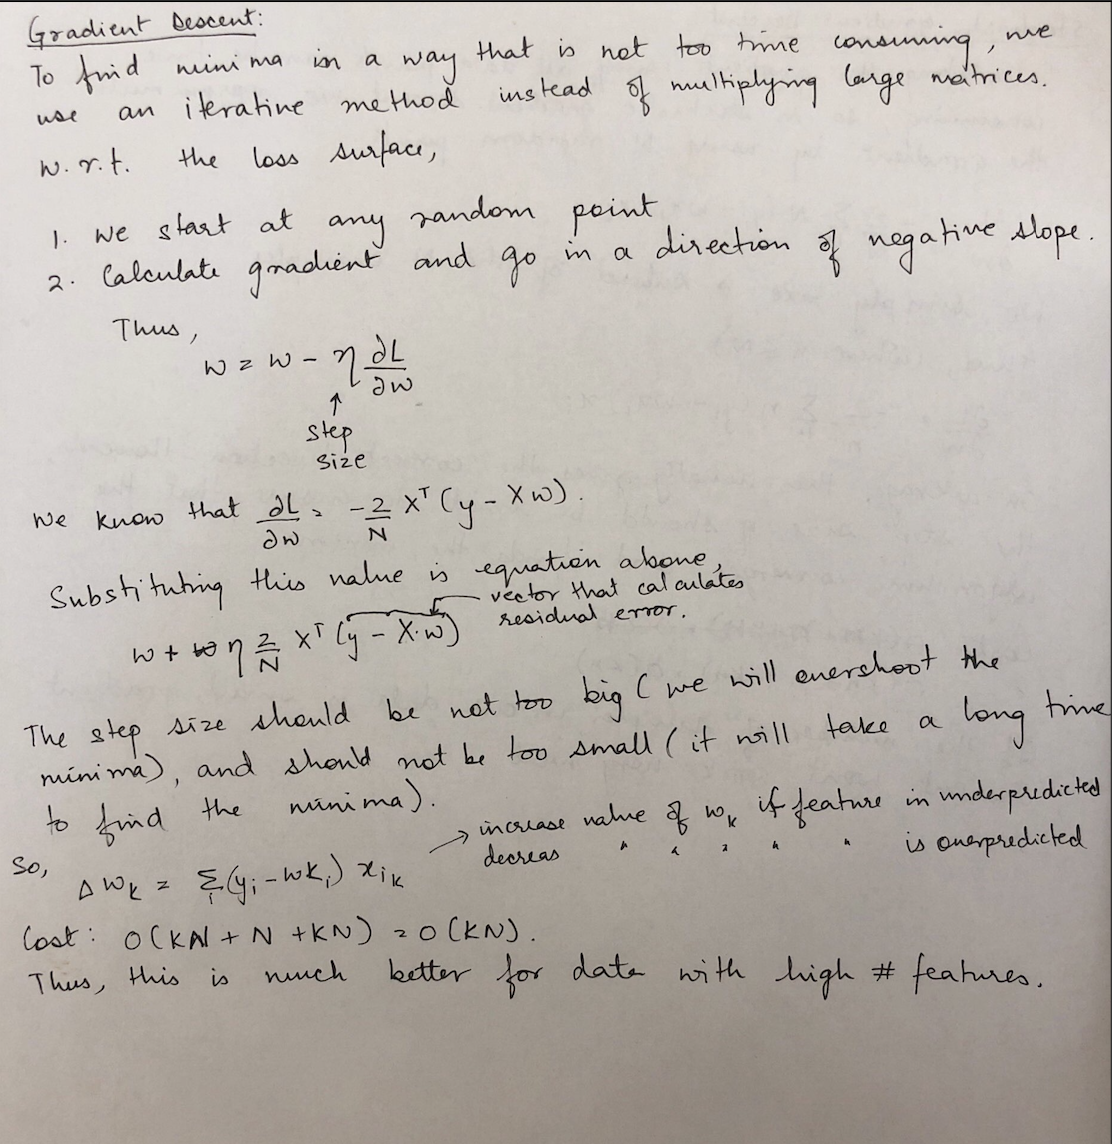
\includegraphics[scale=0.7]{figures/6.png}
    \caption{Gradient Descent }
    \label{fig:6}
  \end{center}
\end{figure}
\newpage
\subsection{Stochastic gradient descent:}

\begin{figure}[!ht]
  \begin{center}
    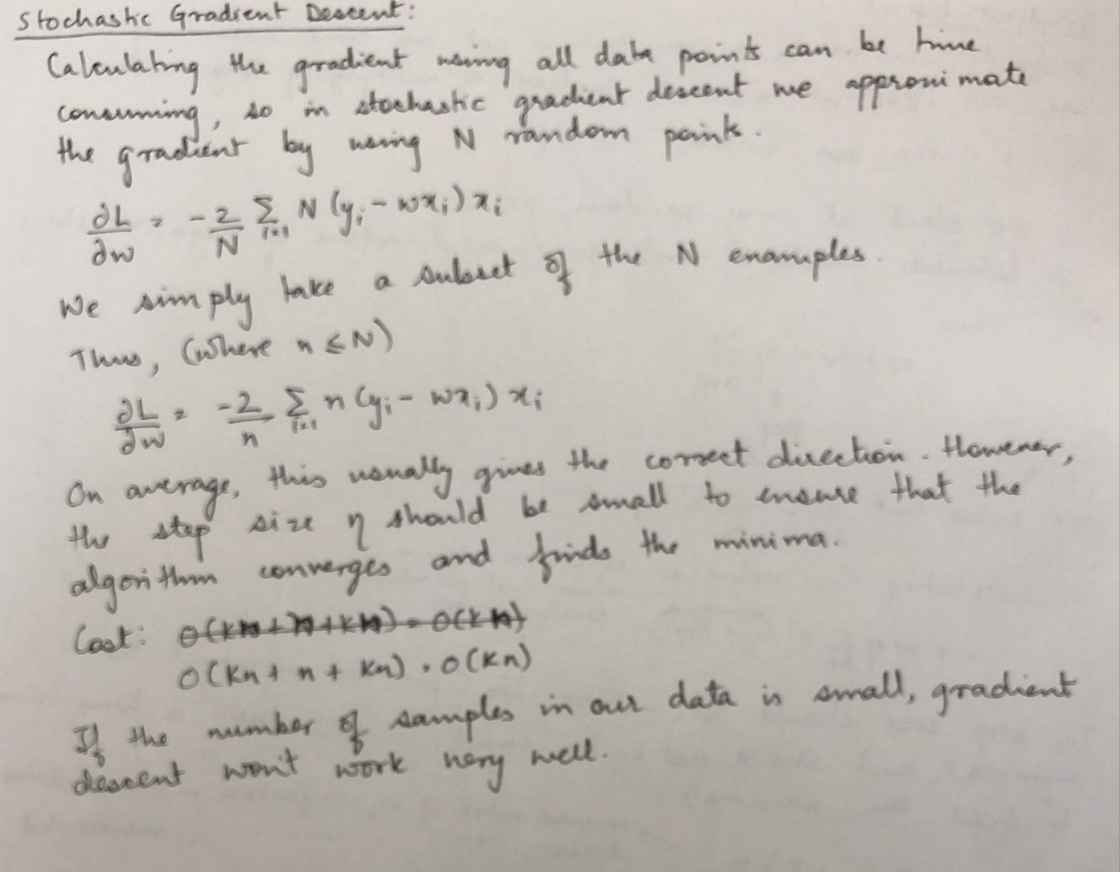
\includegraphics[scale=0.7]{figures/7.png}
    \caption{Stochastic Gradient Descent }
    \label{fig:7}
  \end{center}
\end{figure}

\end{document}

%%% Local Variables:
%%% mode: latex
%%% TeX-master: t
%%% End: